\section{Supły} % (fold)
\label{sec:tangle}

Na przełomie lat sześćdziesiątych i~siedemdziesiątych Conway szukał sposobu na zbudowanie kompletnej tablicy węzłów.
Niezmienniki znane w~tym czasie nie były dostatecznie mocne, by sprostać temu wyzwaniu.
Conway wprowadził pojęcie supła i~chociaż wszystkich węzłów nie można z~nich uzyskać, teoria została pchnięta do przodu.
Supły stanowią budulec splotów takich jak na przykład precle z~definicji \ref{def:pretzel}.

Sekcja oparta jest na podręczniku Murasugiego \cite{murasugi96} i~pracach \cite{conway70}, \cite{kauffman97}, \cite{kauffman04}, a~także \cite{schubert56}.
Po raz pierwszy z~supłami zetknęliśmy się w~pracy \cite{janiak04}, także czerpiącej inspirację z~\cite{murasugi96}, choć podejrzewamy, że konwencje nazewnicze w tych pracach wzajemnie wykluczają się.

\begin{definition}[supeł]
    \label{def:tangle}
    \index{supeł}
    Zawarty w~kole fragment diagramu splotu o~dwóch łukach wyjściowych oraz dwóch wejściowych, nazywamy supłem.
\end{definition}

Istnieją dwa rodzaje supłów -- naprzemienne i~sąsiadujące.
\begin{center}
    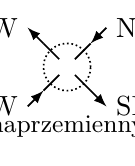
\begin{tikzpicture}[baseline=-0.65ex, scale=0.1]
    \useasboundingbox (-5, -9) rectangle (5, 5);
        \node [left] at (-5, -5) {SW};
        \draw[semithick,latex-] (-3, -3) to (-5,-5);
        \draw[semithick] (-3, -3) to (-1,-1);
        \node [right] at (5, 5) {NE};
        \draw[semithick,latex-] (3, 3) to (5,5);
        \draw[semithick] (3, 3) to (1,1);
        \node [right] at (5, -5) {SE};
        \draw[semithick,-latex] (3, -3) to (5,-5);
        \draw[semithick] (3, -3) to (1,-1);
        \node [left] at (-5, 5) {NW};
        \draw[semithick,-latex] (-3, 3) to (-5,5);
        \draw[semithick] (-3, 3) to (-1,1);
        \draw[semithick, densely dotted] (-0, 0) circle (3);
        \node at (0, -5) [below] {\small naprzemienny};
    \end{tikzpicture}
    \quad\quad\quad\quad\quad\quad
    \begin{tikzpicture}[baseline=-0.65ex, scale=0.1]
    \useasboundingbox (-5, -9) rectangle (5, 5);
        \node [left] at (-5, -5) {SW};
        \draw[semithick,latex-] (-3, -3) to (-5,-5);
        \draw[semithick] (-3, -3) to (-1,-1);
        \node [right] at (5, 5) {NE};
        \draw[semithick,-latex] (3, 3) to (5,5);
        \draw[semithick] (3, 3) to (1,1);
        \node [right] at (5, -5) {SE};
        \draw[semithick,latex-] (3, -3) to (5,-5);
        \draw[semithick] (3, -3) to (1,-1);
        \node [left] at (-5, 5) {NW};
        \draw[semithick,-latex] (-3, 3) to (-5,5);
        \draw[semithick] (-3, 3) to (-1,1);
        \draw[semithick, densely dotted] (-0, 0) circle (3);
        \node at (0, -5) [below] {\small sąsiadujący};
    \end{tikzpicture}
\end{center}

Podobnie jak dla węzłów, pojawia się naturalne pytanie o~równoważność dwóch supłów.
Jest tak wtedy, gdy istnieje homeomorfizm* kuli na siebie, który przekształca jeden supeł na drugi, ale nie rusza sfery otaczającej.
Dla diagramów odpowiada to ruchom Reidemeistera, nie mamy jednak prawa opuszczać kuli zawierającej supeł.

Wszystkich supłów jest bardzo dużo, więc ograniczymy się do końca rozdziału do pewnej ich regularnej rodziny.
Oto cztery podstawowe supły:
\begin{comment}
\[
    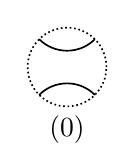
\begin{tikzpicture}[baseline=-0.65ex, scale=0.1]
    \useasboundingbox (-5, -9) rectangle (5, 5);
        \draw[semithick] (-5 / 1.4142, -5 / 1.4142) [in=135, out=45] to (5 / 1.4142, -5 / 1.4142);
        \draw[semithick] (-5 / 1.4142, 5 / 1.4142) [in=-135, out=-45] to (5 / 1.4142, 5 / 1.4142);
        \draw[semithick, densely dotted] (-0, 0) circle (5);
        \node at (0, -5) [below] {$(0)$};
    \end{tikzpicture}
    \quad\quad\quad
    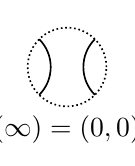
\begin{tikzpicture}[baseline=-0.65ex, scale=0.1]
    \useasboundingbox (-5, -9) rectangle (5, 5);
        \draw[semithick] (-5 / 1.4142, -5 / 1.4142) [in=-45, out=45] to (-5 / 1.4142, 5 / 1.4142);
        \draw[semithick] (5 / 1.4142, -5 / 1.4142) [in=-135, out=135]  to (5 / 1.4142, 5 / 1.4142);
        \draw[semithick, densely dotted] (-0, 0) circle (5);
        \node at (0, -5) [below] {$(\infty) = (0, 0)$};
    \end{tikzpicture}
    \quad\quad\quad
    \begin{tikzpicture}[baseline=-0.65ex, scale=0.1]
    \useasboundingbox (-5, -9) rectangle (5, 5);
    \begin{knot}[clip width=5, end tolerance=1pt]
        \strand[semithick] (-5 / 1.4142, -5 / 1.4142) to (5 / 1.4142, 5 / 1.4142);
        \strand[semithick] (5 / 1.4142, -5 / 1.4142) to (-5 / 1.4142, 5 / 1.4142);
        \strand[semithick, densely dotted] (-0, 0) circle (5);
        \node at (0, -5) [below] {$(-1)$};
    \end{knot}
    \end{tikzpicture}
    \quad\quad\quad
    \begin{tikzpicture}[baseline=-0.65ex, scale=0.1]
    \useasboundingbox (-5, -9) rectangle (5, 5);
    \begin{knot}[clip width=5, end tolerance=1pt, flip crossing/.list={1}]
        \strand[semithick] (-5 / 1.4142, -5 / 1.4142) to (5 / 1.4142, 5 / 1.4142);
        \strand[semithick] (-5 / 1.4142, 5 / 1.4142) to (5 / 1.4142, -5 / 1.4142);
        \strand[semithick, densely dotted] (-0, 0) circle (5);
        \node at (0, -5) [below] {$(1)$};
    \end{knot}
    \end{tikzpicture}
\]
\end{comment}

\begin{definition}
    \label{def:rational_tangle}
    Supły powstające z~$(0)$ lub $(\infty)$ przez homeomorfizm kuli na siebie permutujący wejścia i~wyjścia nazywamy wymiernymi.
\end{definition}

Wystarczy się przy tym ograniczyć do ciągu obrotów półsfery dolnej (SW--SE) oraz lewej (SW--NW)
Z obrotami prawoskrętnymi wiążemy liczby dodatnie, natomiast z~lewoskrętnymi -- ujemne.
Otrzymujemy tak pewną krotkę $(a_1, \ldots, a_n)$.
Jeśli $n$ jest parzyste, zaczynamy od supła $(\infty)$, jeśli nie -- od $(0)$.
Ostatni obrót dotyczy półsfery dolnej.
Krotka nie jest jeszcze niezmiennikiem supłów (gdyż $(-2,3,3) \cong (3, -2, 3)$), ale nic straconego.
Potrzebować będziemy prostej definicji, uzasadniającej określenie ,,supły wymierne''.
% Conway pokazał, że dla dowolnego supła przy pomocy wielomianu Alexandera zdefiniować można  pewien ułamek.

\begin{proposition}
\label{prp:continued_fractions}
    Istnieje bijekcja między klasami supłów wymiernych oraz łańcuchowymi ułamkami, które je przedstawiają:
    \[
        \frac \alpha \beta = a_n + \frac{1}{a_{n-1} + 1 / (a_{n-2} +  \ldots + 1/a_1)} \in \Q \cup \{\infty\}.
    \]
\end{proposition}

\begin{proof}
    Praca \cite{conway70} Conwaya.
\end{proof}

\begin{proposition}
\label{prp:continued_fractions_2}
    Supły o~łańcuchowych ułamkach różnych od $0$ i~$\infty$ można kodować ciągami liczb całkowitych tego samego znaku.
\end{proposition}

Z każdym supłem $T$ związane jest jego odbicie $\overline T$, obraz wyjściowego przez symetrię względem prostej $y = -x$.
Mając dwa supły obok siebie, można dokonać ich sklejenia wzdłuż połówek kul, w~których leżą:
\[
	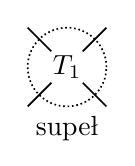
\begin{tikzpicture}[baseline=-0.65ex, scale=0.1]
	\useasboundingbox (-5, -9) rectangle (5, 5);
		\draw[semithick] (-2, -2) to (-5,-5);
		\draw[semithick] (2, 2) to (5,5);
		\draw[semithick] (2, -2) to (5,-5);
		\draw[semithick] (-2, 2) to (-5,5);		%
		\draw[semithick, densely dotted] (-0, 0) circle (5);
		\node at (0, 0) {$T_1$};
		\node [below] at (0, -5) {supeł};
	\end{tikzpicture}
	\quad \quad
	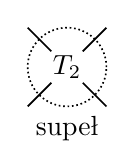
\begin{tikzpicture}[baseline=-0.65ex, scale=0.1]
	\useasboundingbox (-5, -9) rectangle (5, 5);
		\draw[semithick] (-2, -2) to (-5,-5);
		\draw[semithick] (2, 2) to (5,5);
		\draw[semithick] (2, -2) to (5,-5);
		\draw[semithick] (-2, 2) to (-5,5);		%
		\draw[semithick, densely dotted] (-0, 0) circle (5);
		\node at (0, 0) {$T_2$};
		\node [below] at (0, -5) {supeł};
	\end{tikzpicture}
	\quad \quad
	% \begin{tikzpicture}[baseline=-0.65ex, scale=0.1]
	% \useasboundingbox (-15, -9) rectangle (15, 5);
	% 	\draw[semithick] (-12, -2) to (-15,-5);
	% 	\draw[semithick] (-12, 2) to (-15,5);		%
	% 	\draw[semithick, densely dotted] (-10, 0) circle (5);
	% 	\node at (-10, 0) {$T_1$};
	% 	\draw[semithick] (12, -2) to (15,-5);
	% 	\draw[semithick] (12, 2) to (15,5);		%
	% 	\draw[semithick, densely dotted] (10, 0) circle (5);
	% 	\node at (10, 0) {$T_2$};
	% 	\draw[semithick] (-8, 2) [in=135, out=45] to (8, 2);
	% 	\draw[semithick] (-8, -2) [in=-135, out=-45] to (8, -2);
	% 	\node [below] at (0, -5) {produkt};
	% \end{tikzpicture}
	% \quad \quad
	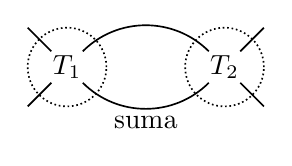
\begin{tikzpicture}[baseline=-0.65ex, scale=0.1]
	\useasboundingbox (-15, -9) rectangle (15, 5);
		\draw[semithick] (-12, -2) to (-15,-5);
		\draw[semithick] (-12, 2) to (-15,5);		%
		\draw[semithick, densely dotted] (-10, 0) circle (5);
		\node at (-10, 0) {$T_1$};
		\draw[semithick] (12, -2) to (15,-5);
		\draw[semithick] (12, 2) to (15,5);		%
		\draw[semithick, densely dotted] (10, 0) circle (5);
		\node at (10, 0) {$T_2$};
		\draw[semithick] (-8, 2) [in=135, out=45] to (8, 2);
		\draw[semithick] (-8, -2) [in=-135, out=-45] to (8, -2);
		\node [below] at (0, -5) {suma};
	\end{tikzpicture}
\]

Oznaczmy tak otrzymany węzeł przez $T_1 + T_2$.
Niektórzy definiują dalsze działania, jak produkt: $T_1 \cdot T_2 = \overline T_1 + T_2$ czy rozgałęzienie, $\overline T_1 + \overline T_2$.
Rodzina supłów wymiernych jest zamknięta na branie produktów, ale nie sum.
Wprowadzamy więc następującą, ogólniejszą definicję.
Supeł będący skończoną sumą supłów wymiernych, ich luster, odbić lub odbić luster nazywamy algebraicznym.

Przez zszycie par łuków wejściowych (lub wyjściowych) zamieniamy supły w~węzły:
\begin{comment}
\[
    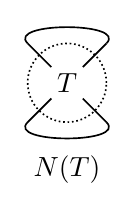
\begin{tikzpicture}[baseline=-0.65ex, scale=0.1]
    \useasboundingbox (-5, -11) rectangle (5, 7);
        \draw[semithick] (-2, -2) to (-5,-5);
        \draw[semithick] (2, 2) to (5,5);
        \draw[semithick] (2, -2) to (5,-5);
        \draw[semithick] (-2, 2) to (-5,5);        %
        \draw[semithick, densely dotted] (-0, 0) circle (5);
        \node at (0, 0) {$T$};
        \node [below] at (0, -8) {$N(T)$};
        \draw[semithick] (-5, -5) [in=-45, out=-135] to (5, -5);        %
        \draw[semithick] (-5,    5) [in=45, out=135] to (5, 5);        %
    \end{tikzpicture}
    \quad \quad
    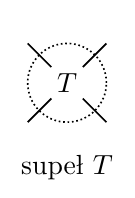
\begin{tikzpicture}[baseline=-0.65ex, scale=0.1]
    \useasboundingbox (-5, -11) rectangle (5, 7);
        \draw[semithick] (-2, -2) to (-5,-5);
        \draw[semithick] (2, 2) to (5,5);
        \draw[semithick] (2, -2) to (5,-5);
        \draw[semithick] (-2, 2) to (-5,5);        %
        \draw[semithick, densely dotted] (-0, 0) circle (5);
        \node at (0, 0) {$T$};
        \node [below] at (0, -8) {supeł $T$};
    \end{tikzpicture}
    \quad \quad
    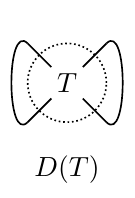
\begin{tikzpicture}[baseline=-0.65ex, scale=0.1]
    \useasboundingbox (-5, -11) rectangle (5, 7);
        \draw[semithick] (-2, -2) to (-5,-5);
        \draw[semithick] (2, 2) to (5,5);
        \draw[semithick] (2, -2) to (5,-5);
        \draw[semithick] (-2, 2) to (-5,5);        %
        \draw[semithick, densely dotted] (-0, 0) circle (5);
        \node at (0, 0) {$T$};
        \node [below] at (0, -8) {$D(T)$};
        \draw[semithick] (-5, -5) [in=135, out=-135] to (-5, 5);        %
        \draw[semithick] (5, -5) [in=45, out=-45] to (5, 5);        %
    \end{tikzpicture}
    \quad \quad
\]
\end{comment}

Oznaczenia $N(T)$ oraz $D(T)$ pochodzą od angielskich słów \emph{numerator}, \emph{denominator}.
Być może nie jest jasne, dlaczego terminy stosowane zazwyczaj do opisu ułamków stosujemy wobec diagramów splotów.
Nazewnictwo nie jest przypadkowe. %, wrócimy do tego tematu wkrótce.
\begin{proposition}
\label{prp:knot_fraction}
    Ułamek supła zadany wzorem
    \[
        F(A) = \frac{\conway_{N(A)}(z)}{\conway_{D(A)}(z)}
    \]
    spełnia zależność $F(A+B) = F(A) + F(B)$.
\end{proposition}

\begin{proof}
    Praca \cite{conway70} Conwaya.
\end{proof}

Istnieją supły $T_1$, $T_2$ takie, że węzły $N(T_i)$ są nietrywialne, ale $N(T_1 + T_2)$ to niewęzeł.
Co gorsza, dla każdego wymiernego supła $A$ istnieje taki supeł $B$, że $N(A+B)$ jest niewęzłem.

Praca \cite{conway70} zawiera jeszcze jeden ciekawy rezultat, uogólniony przez Lickorisha i~Milletta w~\cite{lickorish87}.
Przyjmijmy następujące skróty: niech $A_n = P_{N(A)}(x,y)$, $A_d = P_{D(A)}(x,y)$.

\begin{proposition}
    Dla dowolnych supłów $A, B$ mamy
    \[
    (1 - (x+y)^2)(A+B)_n = (A_nB_d + A_dB_n) - (x+y)(A_nB_n+  A_dB_d)
    \]
    oraz
    \[
        (A+B)_d = A_dB_d.
    \]
\end{proposition}

Uwaga, zastosowano tu nieco inną parametryzację wielomianu HOMFLY.


\subsection{Sploty o~dwóch mostach}
\label{sub:twobridge}%
\index{węzeł!wymierny|see {węzeł dwumostowy}}%
\index{węzeł!dwumostowy|(}%
Zajmiemy się teraz związkiem supłów z liczbą mostową.
Wiemy, że węzeł trywialny jest jednomostowy, następne w hierarchii są sploty dwumostowe.
Nazywa się je także wymiernymi, po angielsku czasami \emph{4-plats}.
Jako pierwszy studiował je Bankwitz z~Schumannem w~1934 roku.
% Kawauchi: as 4-plat presentations, which is just Conway's normal form.
Mają co najwyżej dwie składowe i~są odwracalne \cite[s. 211]{burde14}.

\begin{proposition}
    Sploty dwumostowe są pierwsze.
\end{proposition}

\begin{proof}
    Prosty wniosek z~tego, że liczba mostowa prawie jest addytywna (fakt \ref{prp:bridge_additive}).
\end{proof}

\begin{corollary}
    Pierwsze węzły dwu- lub trzymostowe są albo torusowe, albo hiperboliczne.
\end{corollary}

\begin{proof}
    Kawauchi \cite[s. 130]{kawauchi96} wnioskuje to z twierdzenia, którego nie znamy.
\end{proof}

%\todo[inline]{Murasugi Theorem 9.3.3 (138) lub Janiak-Osajca, Pogoda (34).}
% Aus der unten stehenden Klassifikation ergibt sich, dass man jede Verschlingung mit 2 Brücken wie im Bild rechts darstellen kann, wobei {\displaystyle a_{i}\in \mathbb {Z} } a_{i}\in \mathbb{Z }  die Anzahl der Halbtwists in der jeweiligen Box bezeichnet und für gerade bzw. ungerade {\displaystyle i} i~positive {\displaystyle a_{i}} a_{i} links- bzw. rechtshändigen Halbtwists entsprechen.
% Diese Darstellung wird als Conway-Normalform bezeichnet.
% Man kann stets erreichen, dass alle {\displaystyle a_{i}} a_{i} dasselbe Vorzeichen haben.[1] Insbesondere gibt die Conway-Normalform dann ein alternierendes Knotendiagramm.[2]
%Insbesondere ist ein 2-Brücken-Knoten genau dann amphichiral, wenn {\displaystyle q^{2}\equiv -1\ mod\ p} q^{2}\equiv -1\ mod\ p ist.

\begin{proposition}
    Sploty z~dwoma mostami to dokładnie sploty typu $D(T)$ dla pewnego supła wymiernego $T$.
\end{proposition}

Dowód tego stwierdzenia znaleźć można na przykład w książce \cite{murasugi96}, strony 183-187.
Wynika z niego, że każdy splot dwumostowy można przedstawić następującym diagramem:
\begin{comment}
\[
    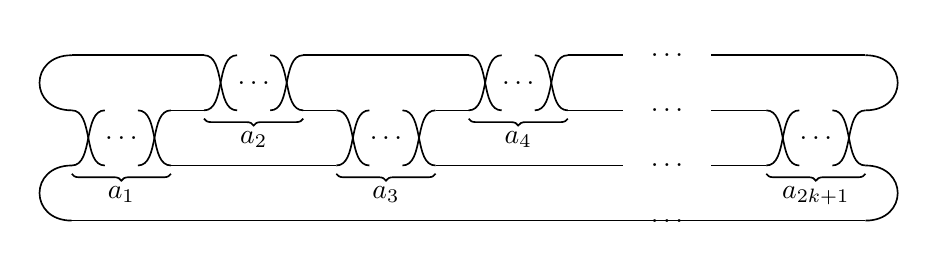
\begin{tikzpicture}[baseline=-0.65ex, xscale=0.14, yscale=0.07]
    \useasboundingbox (-40, -20) rectangle (40, 20);
        %%% A1
        \draw[semithick] (-36, -5) .. controls (-34,-5) and (-35, 5) .. (-33, 5);
        \draw[semithick] (-36,  5) .. controls (-34, 5) and (-35,-5) .. (-33,-5);
        \node at (-31.5, 0) {$\ldots$};
        \draw[semithick] (-30, -5) .. controls (-28,-5) and (-29, 5) .. (-27, 5);
        \draw[semithick] (-30,  5) .. controls (-28, 5) and (-29,-5) .. (-27,-5);
        %%% A2
        \draw[semithick] (-24,  5) .. controls (-22,  5) and (-23, 15) .. (-21, 15);
        \draw[semithick] (-24, 15) .. controls (-22, 15) and (-23,  5) .. (-21,  5);
        \node at (-19.5, 10) {$\ldots$};
        \draw[semithick] (-18,   5) .. controls (-16,  5) and (-17, 15) .. (-15, 15);
        \draw[semithick] (-18,  15) .. controls (-16, 15) and (-17,  5) .. (-15,  5);
        %%% A3
        \draw[semithick] (-12, -5) .. controls (-10,-5) and (-11, 5) .. (-9, 5);
        \draw[semithick] (-12,  5) .. controls (-10, 5) and (-11,-5) .. (-9,-5);
        \node at (-7.5, 0) {$\ldots$};
        \draw[semithick] (-6, -5) .. controls (-4,-5) and (-5, 5) .. (-3, 5);
        \draw[semithick] (-6,  5) .. controls (-4, 5) and (-5,-5) .. (-3,-5);
        %%% A4
        \draw[semithick] (0,  5) .. controls (2,  5) and (1, 15) .. (3, 15);
        \draw[semithick] (0, 15) .. controls (2, 15) and (1,  5) .. (3,  5);
        \node at (4.5, 10) {$\ldots$};
        \draw[semithick] (6,   5) .. controls (8,  5) and (7, 15) .. (9, 15);
        \draw[semithick] (6,  15) .. controls (8, 15) and (7,  5) .. (9,  5);
        %%% A 2k+1
        \draw[semithick] (27,  -5) .. controls (29,  -5) and (28, 5) .. (30, 5);
        \draw[semithick] (27, 5) .. controls (29, 5) and (28,  -5) .. (30,  -5);
        \node at (31.5, 0) {$\ldots$};
        \draw[semithick] (33,   -5) .. controls (35,  -5) and (34, 5) .. (36, 5);
        \draw[semithick] (33,  5) .. controls (35, 5) and (34,  -5) .. (36,  -5);
        %%%    - A3
        \draw[semithick] (-36, 15) to (-24, 15);
        %%% A1 - A3
        \draw[semithick] (-27, -5) to (-12, -5);
        %%% A1 - A2
        \draw[semithick] (-27,  5) to (-24,  5);
        %%% A2 - A3
        \draw[semithick] (-15,  5) to (-12,  5);
        %%% A2 - A4
        \draw[semithick] (-15, 15) to (0, 15);
        %%% A3 - A4
        \draw[semithick] (-3, 5) to (0, 5);
        %%%
        \draw[semithick] ( 9, 15) to (14, 15);
        \draw[semithick] ( 9,  5) to (14,  5);
        \draw[semithick] (-3, -5) to (14, -5);
        \node at (18,  15) {$\ldots$};
        \node at (18,   5) {$\ldots$};
        \node at (18,  -5) {$\ldots$};
        \node at (18, -15) {$\ldots$};
        \draw[semithick] (22, 15) to (36, 15);
        \draw[semithick] (22,  5) to (27,  5);
        \draw[semithick] (22, -5) to (27, -5);
        \draw[semithick] (-36, -15) to (36, -15);
        \draw[semithick] (-36, -15) [in=left,  out=left]  to (-36, -5);
        \draw[semithick] (-36,   5) [in=left,  out=left]  to (-36, 15);
        \draw[semithick] ( 36, -15) [in=right, out=right] to ( 36, -5);
        \draw[semithick] ( 36,   5) [in=right, out=right] to ( 36, 15);
        %
        \draw[semithick, decoration={brace,mirror,raise=3pt},decorate]  (-36, -5) -- node[below=4pt] {$a_1$}      (-27, -5);
        \draw[semithick, decoration={brace,mirror,raise=3pt},decorate]  (-24,  5) -- node[below=4pt] {$a_2$}      (-15,  5);
        \draw[semithick, decoration={brace,mirror,raise=3pt},decorate]  (-12, -5) -- node[below=4pt] {$a_3$}      ( -3, -5);
        \draw[semithick, decoration={brace,mirror,raise=3pt},decorate]  (  0,  5) -- node[below=4pt] {$a_4$}      (  9,  5);
        \draw[semithick, decoration={brace,mirror,raise=3pt},decorate]  ( 27, -5) -- node[below=4pt] {$a_{2k+1}$} ( 36, -5);
    \end{tikzpicture}
\]
\end{comment}

Oto reguła, zgodnie z~którą wybieramy znaki liczb $a_i$:
jeśli $i$ jest nieparzyste, prawy skręt jest dodatni, jeśli parzyste -- lewy jest dodatni.
Sam diagram oznaczamy $C(a_1, \ldots, a_{2k+1})$ i~nazywamy postacią normalną Conwaya.

\begin{proposition}
    % Murasugi proposition 9.3.2
    Sploty dwumostowe są alternujące.
\end{proposition}

\begin{proof}
    Goodrick w~\cite{goodrick72} podał diagramatyczny dowód, gdzie ciąg ruchów zmienia diagram splotu dwumostowego w~alternujący.
    Wynika to też z faktu \ref{prp:continued_fractions}.
    % Burde, Zieschang 2013, strona 217, nazywają to twierdzeniem Bankwitza-Schumanna.
\end{proof}

Przez analogię do supłów, definiujemy ułamek łańcuchowy
\begin{equation}
    C(a_1, \ldots, a_{2k+1}) \mapsto a_1 + \frac{1}{a_2 + 1/\ldots} = \frac \alpha \beta.
\end{equation}

\begin{tobedone}
\index{postać normalna!Conwaya}%
\index{postać normalna!Schuberta}%
    To jest postać normalna Conwaya, ale mamy jeszcze postać Schuberta - \cite[s. 21]{kawauchi96}.
\end{tobedone}

Zauważmy, że wartość bezwzględna ułamka $\alpha/\beta$ zawsze przekracza $1$ i~odwrotnie, każdy taki ułamek pochodzi od pewnego węzła dwumostowego.
Parę względnie pierwszych liczb $(\alpha, \beta)$ nazywamy typem węzła dwumostowego.

\begin{proposition}
    \label{prp:tangle_equivalence}
    Dwumostowe sploty typów $(\alpha, \beta)$ oraz $(\alpha', \beta')$ są, pomijając orientację, równoważne wtedy i~tylko wtedy, gdy spełniony jest jeden z warunków:
    \begin{itemize}
        \item $\alpha = \alpha'$ oraz $\beta \equiv \beta' \pmod \alpha$,
        \item $\alpha = \alpha'$ oraz $\beta \beta' \equiv 1 \pmod \alpha$.
    \end{itemize}
\end{proposition}

% Burde, Zieschang 2013: strona 212, dowód tego.

\begin{tobedone}
    \cite[s. 23]{kawauchi96}: czasem $2\alpha$ zamiast $\alpha$.
\end{tobedone}

\begin{proof}
    Dowód opiera się na tym, że podwójnie cykliczna przestrzeń nakrywająca rozcięta wzdłuż splotu jest przestrzenią soczewkową typu $(\alpha, \beta)$.
    Nie definiowaliśmy nawet tych przestrzeni, szczegóły można znaleźć w~podręczniku \cite{murasugi96} albo \cite{schubert56}.
\end{proof}

\begin{proposition}
    Dwumostowy splot typu $(\alpha, \beta)$ jest achiralny dokładnie wtedy i tylko wtedy, gdy
    \begin{equation}
        \beta^2 \equiv -1 \mod \alpha.
    \end{equation}
\end{proposition}

\begin{proof}
    Wynika to z tego, że lustrem splotu typu $(\alpha, \beta)$ jest splot typu $(\alpha, -\beta)$ oraz faktu \ref{prp:tangle_equivalence}.
\end{proof}

\begin{proposition}
    Niech $b$ będzie dowolną liczbą całkowitą.
    Wtedy następujące sploty są tego samego typu:
    \begin{align}
        N(T(a_1, a_2, \ldots, a_{2k+1})) & \approx N(T(a_1, a_2, \ldots, a_{2k+1}, b, 0)) \\
                                         & \approx D(T(-a_1, -a_2, \ldots, -a_{2k+1}, b)) \\
                                         & \approx C(a_1, a_2, \ldots, a_{2k}-1, 1). \\
        N(T(a_1, a_2, \ldots, a_{2k}))   & \approx D(T(-a_1, -a_2, \ldots, -a_{2k}, b)) \\
                                         & \approx C(a_1, a_2, \ldots, a_{2k}-1, 1). \\
        D(T(a_1, a_2, \ldots, a_{2k+1})) & \approx D(T(a_1, a_2, \ldots, a_{2k}, 0)) \\
                                         & \approx C(1, a_1-1, a_2, \ldots, a_{2k}). \\
        D(T(a_1, a_2, \ldots, a_{2k}))   & \approx D(T(a_1, a_2, \ldots, a_{2k-1}, 0)) \\
                                         & \approx C(a_1, a_2, \ldots, a_{2k-1}).
    \end{align}
\end{proposition}

\begin{proof}
    \cite[fakt 9.3.4]{murasugi96}
\end{proof}

\begin{proposition}
    Niech $L$ będzie dwumostowym splotem typu $(\alpha, \beta)$.
    Wtedy $\det L = \alpha$.
\end{proposition}

Wynika stąd, że wyznacznik nie wystarcza do odróżniania splotów dwumostowych.

\begin{proof}
    % Chcąc oszczędzić niektórym Czytelnikom cierpień odsyłamy po prostu do \cite{schubert56}.
    \url{https://math.stackexchange.com/questions/3327846/}.
\end{proof}

Niech $A, B$ będą supłami.
Wiemy, że suma $A+B$ nie musi być supłem, zaś $D(A+B)$ niekoniecznie jest splotem dwumostowym.
Pomimo to, splot $N(A+B)$ jest dwumostowy, potrafimy nawet powiedzieć, jaki ma wyznacznik:

\begin{proposition}
    % Theorem 9.3.5 Murasugi

    Niech $A, B$ będą supłami, którym odpowiadają skrócone ułamki $p/q$ oraz $r/s$.
    Wtedy splot $L = N(A+B)$ jest dwumostowy, typu $(\alpha, \beta)$ i ma wyznacznik $\alpha = |ps + qr|$.
\end{proposition}

Murasugi (twierdzenie 9.3.5) twierdzi, że dowód znajduje się u Ernsta, Sumnersa \cite{ernst90}.
\index[persons]{Ernst, Claus}%
\index[persons]{Sumners, De Witt}%

\begin{proposition}
    Rozpatrzmy węzeł dwumostowy typu $(\alpha, \beta)$, gdzie $0 < \beta < \alpha$ i~$\beta$ jest nieparzyste.
    Niech $r_k$ będzie resztą z~dzielenia $k\beta$ przez $2\alpha$ leżącą w~przedziale $(-\alpha, \alpha)$ dla $k = 0, 1, \ldots, \alpha - 1$.
    Różnica między ilością dodatnich reszt i~ujemnych reszt to sygnatura węzła.
\end{proposition}

Wygląda na to, że jedynym niewyznaczonym do końca klasycznym niezmiennikiem jest liczba gordyjska.

\index{węzeł!dwumostowy|)}%

% Koniec podsekcji Sploty o~dwóch mostach




\subsection{Mutanty i mutacje}
\index{mutant|(}%
\index{mutacja|see {mutant}}%
\label{sec:mutant}%
Na zakończenie wspomnimy o~mutacjach.

\begin{definition}[mutacja]
    % \labelnotinuse{def:mutacja}
    Półobrót supła względem osi poziomej, pionowej albo też prostopadłej do płaszczyzny, w~jakiej leży diagram, nazywamy mutacją.
    W razie potrzeby zmieniamy orientację supła na przeciwną.
\end{definition}

\begin{definition}[mutant]
\label{def:mutant}%
    Niech $K$ będzie węzłem.
    Węzeł, który powstaje przez ciąg mutacji na węźle $K$, nazywamy mutantem węzła $K$.
\end{definition}

Mutacja węzła o~co najwyżej dziesięciu skrzyżowaniach nie zmienia jego klasy abstrakcji.
Najprostszą, a zarazem najsłynniejszą parą różnych od siebie mutantów stanowią węzeł Conwaya $11n_{34}$ oraz Kinoshity-Terasakiego $11n_{42}$.
\index{węzeł!Conwaya}%
\index{węzeł!Kinoshity-Terasakiego}%

Conway zauważył podczas klasyfikacji niealternujących węzłów, że tylko one posiadają trywialny wielomian Alexandera.
Mają też taki sam wielomian Jonesa,
\begin{equation}
    \jones(t) = t^{6} -2t^5 +2t^4 -2t^3 +t^2 +2t^{-1} -2t^{-2} +2t^{-3} -t^{-4}.
\end{equation}

Kinoshita, Terasaki \cite{kinoshita1957} zdefiniowali nieskończoną rodzinę węzłów, której pierwszym wyrazem jest węzeł $11n_{42}$ (i wszystkie mają trywialny wielomian Alexandera).
\index[persons]{Kinoshita, Shinichi}%
\index[persons]{Terasaka, Hidetaka}%
Dowód tego, że $11n_{34}$ oraz $11n_{42}$ są różne, jako pierwszy podał prawdopodobnie Riley w~1971 roku \cite{riley1971}: wykorzystał on homomorfizmy z~grupy węzła w~$PSL(2, 7)$.
\index[persons]{Riley, Robert}%
%=% "The inequivalence of these knots was first observed by [Riley 1971]." - Kawauchi, strona 44
Genusy, odpowiednio: $3$ i~$2$, wyznaczył Gabai piętnaście lat później w~\cite{gabai1986}, używał foliacji.
\index[persons]{Gabai, David}%


\begin{figure}[H]
    \centering
    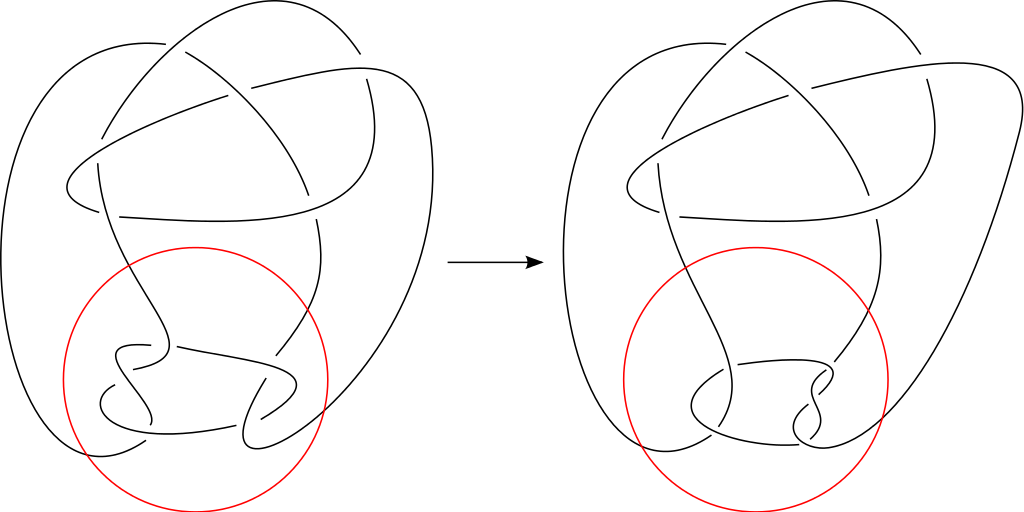
\includegraphics[width=0.601\linewidth]{../data/mixed/knudemutation.png}
    \caption{Węzły $11n_{42}$ oraz $11n_{34}$. Grafika Sørena Jørgensena, dostępna na licencji \href{https://creativecommons.org/licenses/by-sa/3.0/deed.en}{CC BY-SA 3.0} pod adresem \url{https://en.wikipedia.org/wiki/File:Knudemutation.svg}.}
\end{figure}
    
Niedawno Stojmenow podjął się systematycznie szukania mutantów wśród węzłów o~mniej niż 19 skrzyżowaniach (praca \cite{stoimenow2010} z~2010 roku).
\index[persons]{Stojmenow, Aleksander}%
Początkowo pracował sam, badając pewne subtelne przykłady postanowił uwikłać w swój projekt Toshifumiego Tanakę, a później także Daniela Mateię.
\index[persons]{Tanaka, Toshifumi}%
\index[persons]{Daniel, Matei}%
Praca \cite{stoimenow2010} jest kontynuacją artykułu, który napisali wspólnymi siłami.

I tak na stronie 531 można przeczytać, że ,,niezmienniki Wasiljewa co najwyżej 8. stopnia nie rozróżniają mutantów węzłów \cite{chmutov1994}'', ja tego nie widzę.
\index{niezmiennik!Wasiljewa}%
Mniej więcej sześć lat później wynik poprawił J. Murakami (nie mylić z H. Murakamim!) do 10. stopnia w~niezindeksowanej pracy \cite{murakami1999}.
\index[persons]{Murakami, Jun}
W międzyczasie Cromwell, Morton znaleźli niezmiennik stopnia 11., który odróżnia węzły Conwaya oraz Kinoshity-Terasakiego; patrz \cite{cromwell1996}.
\index[persons]{Cromwell, Peter}%
\index[persons]{Morton, Hugh}%
% czy Murakami potwierdził wynik Cromwella, Mortona?

Mutant węzła złożonego także jest złożony, co więcej istnieje bijekcja między czynnikami w ich rozkładach na węzły pierwsze Ruberman -- \cite{ruberman1987}.
\index[persons]{Ruberman, Daniel}%
Dzięki temu możemy bez straty ogólności założyć, że badamy tylko węzły pierwsze, niestety wciąż nie jest znana ogólna procedura pozwalająca wyliczyć wszystkie mutanty danego węzła.

Zaraz po rewolucji, jaką w latach 80. wywołała relacja kłębiasta, Ewing napisał z~Millettem komputerowy program w~języku C, który wyjątkowo szybko znajdował wielomiany HOMFLY oraz Kauffmana zadanego węzła.
\index[persons]{Ewing, Bruce}%
\index[persons]{Millett, Kenneth}%
Nawet dziś program ten jest w stanie uporać się z węzłami, z którymi nie radzą sobie inne narzędzia.
Autorzy nie wiedzieli wtedy, że ktoś jeszcze będzie z nich korzystać w przyszłości, dlatego poczynili w kodzie liczne optymalizacje dla stacji roboczej Sun, jaką wtedy dysponowali.
Dzisiaj okazuje się, że dla węzłów o większej liczbie skrzyżowań program często kończy swoje działanie zrzutem pamięci, wpada w pętlę bez wyjścia albo zwraca niepoprawny wynik (składniki wielomianu Kauffmana są postaci $a^m z^n$, gdzie $m + n$ jest nieparzyste).
Stojmenow korzystał z tych programów podczas tablicowania mutantów.
Jak postępował?
\begin{enumerate}
    \item podzielił węzły na grupy o tej samej objętości, wielomianie Jonesa oraz Alexandera;
    \item w każdej z grup szukał ciągu mutacji pomiędzy diagramami minimalnymi;
    \item tam, gdzie nie udało się znaleźć mutantów, liczył 2-kablowy wielomian HOMFLY;
    \item jeśli wielomian był taki sam, szukał ciągu mutacji między nieminimalnymi diagramami do 18 skrzyżowań;
    \item wreszcie pozostałe grupy zostały potraktowane reprezentacjami grupy podstawowej dwukrotnego nakrycia.
\end{enumerate}

Podsumowanie jego pracy zawiera tabela:

\begin{table}[H]
    \centering
    \begin{tabular}{lccccc} \toprule
        skrzyżowania & 11 & 12 & 13  & 14   & 15    \\ \midrule
        pary         & 16 & 70 & 703 & 3917 & 24884 \\
        trójki       &    & 5  & 38  & 233  & 1000  \\
        czwórki      &    &    & 32  & 262  & 2909  \\
        szóstki      &    &    & 1   & 17   & 172   \\
        ósemki       &    &    &     & 6    & 84    \\
        łącznie      & 16 & 75 & 774 & 4435 & 29049 \\
        \bottomrule
        \hline
    \end{tabular}
    \caption{Liczba grup mutantów wśród pierwszych węzłów do 15 skrzyżowań}
\end{table}

\subsubsection{Rozróżnianie mutantów}
Żaden wielomianowy niezmiennik opisany w~tej książce nie potrafi odróżnić od siebie węzłów $11n_{34}$ oraz $11n_{42}$.
Okazuje się, że niewielomianowe niezmienniki też często są bezradne.

\begin{proposition}
    Mutacja węzła nie zmienia jego wielomianu Alexandera.
\index{wielomian!Alexandera}%
\end{proposition}

% w commicie 1fe48ad183cb592e897f4151f9c18439baa84274 wymieniam:
% +    kablowego wielomianu Jonesa, % menasco91
% +    2-kablowego wielomianu HOMFLY, % przytycki89
% +    kablowego wielomianu Kauffmana, % lipson87
% +    sygnatury Tristrama-Levine'a, % cooper99
% +    symplicjalnEj objętości Gromowa, % ruberman87
% +    instanton homologii Floera, % ruberman99
% +    niezmienników Wittena % rong94
% +    ani Cassona. % kirk89
% ale teraz nie potrafię sobie przypomnieć, jak znalazłem te niezmienniki/prace. :(
% wydaje mi się, że źródłem nie jest stoimenow10, może Math Overflow?

\begin{proof}
    Stojmenow, Tanaka \cite[s. 1]{tanaka2009} piszą, że to proste ćwiczenie teorii kłębiastej, oraz że rozumowanie łatwo przenosi się na odkryte później wielomiany Jonesa, HOMFLY, BLM/Ho, Kauffmana.
\end{proof}

Warto przytoczyć teraz obserwację 3.8.2 z \cite[s. 43]{kawauchi1996} pochodzącą tak naprawdę z pracy Viro \cite{viro1973}: niech sploty $L_1, L_2$ będą mutantami, wtedy podwójne przestrzenie nakryciowe nad $S^3$ rozgałęzione wzdłuż $L_1$ albo $L_2$ są homeomorficzne z zachowaniem orientacji.
Cooper \cite{cooper1982} zauważył, że macierze Seiferta mutantów są $S$-równoważne.
\index{macierz!Seiferta}%
To tłumaczy czemu większość niezmienników nie radzi sobie z odróżnianiem mutantów.
% Viro: Two-fold branched coverings of three-sphere

% z tanaka09
Wzór kablowy\footnote{Niech $T$ będzie trywialnym torusem, zawierającym węzeł $K$, zaś $e \colon T \to S^3$ włożeniem $T$ na otoczenie węzła $C$ tak, że $e$ przenosi równoleżnik $T$ na równoleżnik $C$. Wtedy $\alexander_{eK} (t) = \alexander_K(t)\alexander_C(t^n)$.} \cite[tw. 6.15]{lickorish1997} pokazuje, że wielomian Alexandera nie odróżnia satelitów zmutowanych węzłów.
Wielomian Jonesa nie spełnia żadnego wzoru kablowego (gdyż czasami odróżnia kable węzłów o~tym samym wielomianie), ale…
\index{wzór!kablowy}%

\begin{proposition}
    Mutacja węzła nie zmienia jego kablowego wielomianu Jonesa.
\index{wielomian!Jonesa}%
\end{proposition}

\begin{proof}
\index[persons]{Morton, Hugh}%
\index[persons]{Traczyk, Paweł}%
    Morton, Traczyk \cite{traczyk1988}.
    % kiedyś tu było niezdefiniowane menasco91 = Menasco, Thistlethwaite: The Tait flyping conjecture, ale w 2022 roku przeczytałem Stoimenow: Tabulating and distinguishing mutants zmieniłem zdanie: "nonetheless Morton and Traczyk [36] showed that..."
\end{proof}

Praca \cite{traczyk1988} wspomina jeszcze, że to samo jest prawdą także dla ,,wielomianu Jonesa dwóch zmiennych'' (HOMFLY) i 2-kabli, ale nie dla dowolnych satelitów.
Fakt, że wielomian HOMFLY (a także Kauffmana) nie odróżniają 2-satelitów mutantów, odkryto rok wcześniej:

\begin{proposition}
\label{mutants_and_homfly}%
\index{wielomian!HOMFLY}%
    Mutacja węzła nie zmienia jego 2-kablowego wielomianu HOMFLY.
\end{proposition}

\begin{proof}
\index[persons]{Lickorish, William}%
\index[persons]{Lipson, Andrew}%
\index[persons]{Przytycki, Józef}%
    Lickorish, Lipson \cite{lipson1987}, później też Przytycki \cite{przytycki1989}.
    % TODO: skąd to o Przytyckim???
\end{proof}

Lepiej jest z~3-kablami: wielomian HOMFLY odróżnia tak węzły Kinoshity-Terasakiego i~Conwaya, ale wymaga takiej ilości rachunków, że mało komu chce się je przeprowadzać dla innych węzłów.
\index{węzeł!Conwaya}%
\index{węzeł!Kinoshity-Terasakiego}%

\begin{proposition}
    Mutacja węzła nie zmienia jego (2-?)kablowego wielomianu Kauffmana.
\index{wielomian!kablowy}%
\index{wielomian!Kauffmana}%
\end{proposition}

\begin{proof}
\index[persons]{Lickorish, William}%
\index[persons]{Lipson, Andrew}%
    Lickorish, Lipson \cite{lipson1987}.
\end{proof}

Morton w recenzji pracy Lickorisha, Lipsona wspomina, że dla satelitów owijających się więcej niż $2$ razy to nie jest prawda, jak później odkryto.

\begin{proposition}
\index{wielomian!BLM/Ho}%
    Mutacja węzła nie zmienia jego wielomianu BLM/Ho.
\end{proposition}

\begin{proof}
    \cite{tanaka2009}, choć nie wiemy, gdzie dokładnie.
\end{proof}

\begin{proposition}
\index{sygnatura!Levine'a-Tristrama}%
    Mutacja węzła nie zmienia jego sygnatury Levine'a-Tristrama.
\end{proposition}

\begin{proof}
\index[persons]{Cooper, Daryl}%
\index[persons]{Lickorish, William}%
    Cooper, Lickorish w~\cite{cooper1999} podają klasyczny dowód, że mutacja zachowuje wielomian Alexandera, oparty o~macierz Seiferta.
    Wiedząc, jak wygląda ta macierz, autorzy wyciągają wniosek, że sygnatura splotów (!) w~homologicznej 3-sferze też jest zachowywana.
\end{proof}

\begin{proposition}
\index{objętość!symplicjalna Gromowa}%
\label{mutants_the_same_volume}%
    Mutacja węzła nie zmienia jego symplicjalnej objętości Gromowa.
\end{proposition}

\begin{proof}
\index[persons]{Ruberman, Daniel}%
    Ruberman \cite{ruberman1987}.
    % Ruberman [42] showed that mutants have equal volume in all hyperbolic pieces of the JSJ decomposition.
\end{proof}

\begin{proposition}
\index{homologia!Floera}%
    Mutacja węzła nie zmienia jego instanton homologii Floera.
\end{proposition}

\begin{proof}
\index[persons]{Ruberman, Daniel}%
    Jeszcze raz Ruberman \cite{ruberman1999}.
\end{proof}

\begin{proposition}
\index{niezmiennik!Wittena}%
    Mutacja węzła nie zmienia jego niezmienników Wittena.
\end{proposition}

\begin{proof}[Niedowód]
    Rong \cite{rong1994}: niech $L$ będzie obramowanym splotem w~3-rozmaitości $M$, zaś $F \subseteq M$ dwustronną powierzchnią, tnącą splot w 0, 1 lub 4 (transwersalnie) punktach, o genusie $g = 0$, $1$ lub $2$, wtedy rozcięcie $M$ wzdłuż $F$ i sklejenie po obrocie o 180 stopni daje parę $(M^\tau, K^\tau)$, która ma ten sam niezmiennik Wittena w $\mathrm{SU}(2)$ jak wyjściowa para $(M, K)$.
    % TODO: dla wybranych mutacji
\end{proof}

\begin{proposition}
\index{niezmiennik!Cassona}%
    Mutacja węzła nie zmienia jego niezmienników Cassona.
\end{proposition}

Celowo nie podajemy definicji tego niezmiennika.
Nieformalnie, zlicza on co drugą klasę sprzężoności reprezentacji grupy podstawowej homologicznej 3-sfery w grupie $SU(2)$.

\begin{proof}
\index[persons]{Kirk, Paul}%
    Kirk \cite{kirk1989}.
\end{proof}

\begin{conjecture}
    Mutacja węzła nie zmienia jego liczby gordyjskiej.
\end{conjecture}

Jak czytamy w \cite[problem 1.69]{kirby1978}, przypuszczenie to jest bardzo trudne do udowodnienia, bo wynikałaby z niego bardzo stara hipoteza \ref{conjecture_unknotting_additive}, że liczba gordyjska splotów jest addytywna.
\index{hipoteza!o liczbie gordyjskiej}%
Przytoczymy dwa częściowe wyniki.
Najpierw Rolfsen \cite{rolfsen1993} zauważył, że jedynym mutantem niewęzła jest sam niewęzeł.
\index[persons]{Rolfsen, Dale}%
Dekadę później Gordon, Luecke \cite{gordon2006} pokazali, iż klasa węzłów $1$-gordyjskich jest zamknięta na przeprowadzanie mutacji.
\index[persons]{Gordon, Cameron}%
\index[persons]{Luecke, John}%
(Ohtsuki \cite[problem 12.15]{ohtsuki2002} powtarza hipotezę.)
\index[persons]{Ohtsuki, Tomotada}%

% to NIE jest z stoimenow10
\begin{proposition}
    Niech $D$ będzie alternującym diagramem.
    Wtedy każdy mutant $D$ też jest alternujący.
\end{proposition}

Wśród niezmienników, które mutacja czasami zmienia, znajduje się genus plastrowy:

\begin{proposition}
\index{genus!plastrowy}%
    Niech $m, n$ będą nieujemnymi liczbami całkowitymi.
    Wtedy istnieje węzeł $K$ o genusie plastrowym równym $m$, którego pewien mutant ma genus plastrowy równy $n$.
\end{proposition}

Stanowi to uogólnienie obserwacji Livingstona \cite{livingston1983}, że istnieją mutanty o~różnym genusie plastrowym.
\index[persons]{Livingston, Charles}%

\begin{proof}
    Kim, Livingston w \cite{kim2005}.
\end{proof}

Zbiór problemów niskowymiarowej topologii opublikowany przez Kirby'ego \cite{kirby1978} zawiera następujące pytanie:
\index[persons]{Kirby, Rob}%

\begin{conjecture}[problem 1.91]
\index{węzeł!satelitarny}
    Niech $K$ będzie prostym węzłem bez orientacji (w jego dopełnieniu nie ma nierównoległych do brzegu, nieściśliwych pierścieni).
\index{nieściśliwy}%
    Czy istnieją węzły niebędące mutantami $K$, których nie można odróżnić od $K$ wielomianem Jonesa oraz wszystkimi jego satelitami?
\end{conjecture}

Stojmenow pisze, że tak: pierwszą chronologicznie parą jest $14_{41721}$, $14_{42125}$, dowód opiera się na wzorze fuzyjnym Masbauma-Vogela z~pracy \cite{masbaum1994}.
\index[persons]{Stojmenow, Aleksander}
\index[persons]{Masbaum, Gregor}%
\index[persons]{Vogel, Pierre}%
\index{wzór!fuzyjny Masbauma-Vogela}%
Patrz \cite[przykład 3.3]{tanaka2009} oraz \cite[przykład 3.2]{stoimenow2010}.

Choć wzór ten zastosowany do konkretnej pary węzłów sprawia zazwyczaj trudności rachunkowe, to jest wystarczającym narzędziem, by rozszerzyć konstrukcję do ogólnego wyniku:

\begin{proposition}
    Istnieje nieskończenie wiele par prostych węzłów hiperbolicznych o tych samych kolorowych wielomianach Jonesa, które nie są swoimi mutantami.
\end{proposition}

\begin{proof}
    Stojmenow, Tanaka \cite[tw. 1.1]{tanaka2009}.
\end{proof}

\index{mutant|)}



% Koniec sekcji Supły
